\chapter{Conceito do projeto}
\label{chap:fundteor}

Para a realização de cada desafio foi necessario capitar conhecimento de diversas fontes para poder construi-lo. Contudo fica evidente a necessidade de trazer esses materiais que inspiraram a produção de tal material.

\section{Desafio Workbooks Python}

O desafio de Workbooks utilizando a linguagem python foi composto de 16 desafios de programação utilizando a linguagem python. Partindo dessa contexto, tudo se iniciou com o estudo de bibliotecas e python, para poder ralizar as tarefas da forma mais eficiente possivel.

\section{Desafio C++}
O desafio de C++ foi composto de três desafios de programação que utiliza a linguagem de programação C++. Portanto para a primeira tarefa foi feito um estudo matematico para a enteder como funciona o triangulo de pascal. Em seguida para a segunda tarefa foi feito um estudo combinatorio sobre permutações e depois um estudo sobre bibliotecas  com a função de realizar essas combinações de palavras de forma mais eficaz. Por fim, para a terceira foi feito um estudo acerca de bibliotecas que trabalhassem com arquivos para assim ler o codigo que estava escrito. Dessa maneira, foram baseados a construção dos desafios.

\section{Turtlesim setpoint position}
Consiste em utilizar o software \textit{Turtlesim} para através do ROS escolher uma posição e fazê-lo se deslocar até ela. A movimentação programada na \textit{Turtlesim} se baseia em uma teoria principal, que é o \textit{Dead Reckoning}. Dessa forma, o \textit{Dead Reckoning} consiste em calcular a distância que falta do robô para determinado objetivo e incorporar esses valores a sua posição e velocidade, como pode ser exemplificado na figura \ref{fig:Dead reckoning}. No caso da \textit{Turtlesim} foi calculado sua distância usando o teorema de pitágoras e o ângulo pelo qual a tartaruga precisou virar pela trigonometria.

%imagem  https://en.wikipedia.org/wiki/Dead_reckoning

\begin{figure}[h!]
    \centering
    \caption{Dead reckoning}
    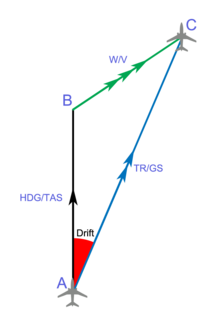
\includegraphics[width=0.4\textwidth]{Figures/dead_reck.png}
    \caption*{Fonte: Wikipedia.}
    \label{fig:Dead reckoning}
\end{figure}

Na navegação do \textit{Turtlesim}, o teorema de pitagoras é utilizado para calcular
a distância entre a mesma e o objetivo definido durante cada instante. Para isso foi utilizado a fórmula 
    $d = \sqrt{(x\textsubscript{f} - x\textsubscript{i})^2 + (y\textsubscript{f} - y\textsubscript{i})^2}$
. Nos quais x\textsubscript{f} e y\textsubscript{f} são as distâncias finais e x\textsubscript{i} e y\textsubscript{i} são as distâncias da tartaruga em determinado instante.

Assim, para calcular quanto que o \textit{Turtlesim} precisa girar faz o uso da trigonometria, para calcular o ângulo do qual a \textit{Turtlesim} esta deslocada  em relação ao objetivo. Com isso, se faz o uso da fórmula de arctg na qual 
$\theta = \frac{y\textsubscript{f} - y\textsubscript{i}}{x\textsubscript{f} - x\textsubscript{i}} $
. Por fim, pegamos esse angulo e subtraímos do ângulo atual da \textit{Turtlesim} para descobrir o quanto a tartaruga precisa rotacionar.

Para definir a velocidade da tartaruga multiplicamos a distância por uma constante e para descobrir o quanto ela precisa rotacionar multiplicamos a 
angulação por outra constante. Assim esses dados são publicados no topic
cmd\_vel para alterar a velocidade da turtle até que ela chegue no objetivo
especificado.

\section{Desafio Webots}

O Webots é uma plataforma opensource usada para simular robôs. 
Desse modo, o desafio consiste em utilizar essa plataforma para 
simular um robo chamado piooner3x, corrigindo o código ja existente
e alterando ele para caso ele encontre uma luminaria pare de se locomover.

A partir disso foram realizados os tutoriais dessa plataforma para 
ter conhecimento de como utilizá-la e como simular os robôs. 
Em seguida foi colocado um sensor de luz no piooner3x para que 
o mesmo tenha uma forma de detectar a luminosidade do ambiente
e seu código foi alterado para que se a leitura do sensor 
ultrapasse determinado valor ele pare.

\begin{figure}[h!]
    \centering
    \caption{Webots}
    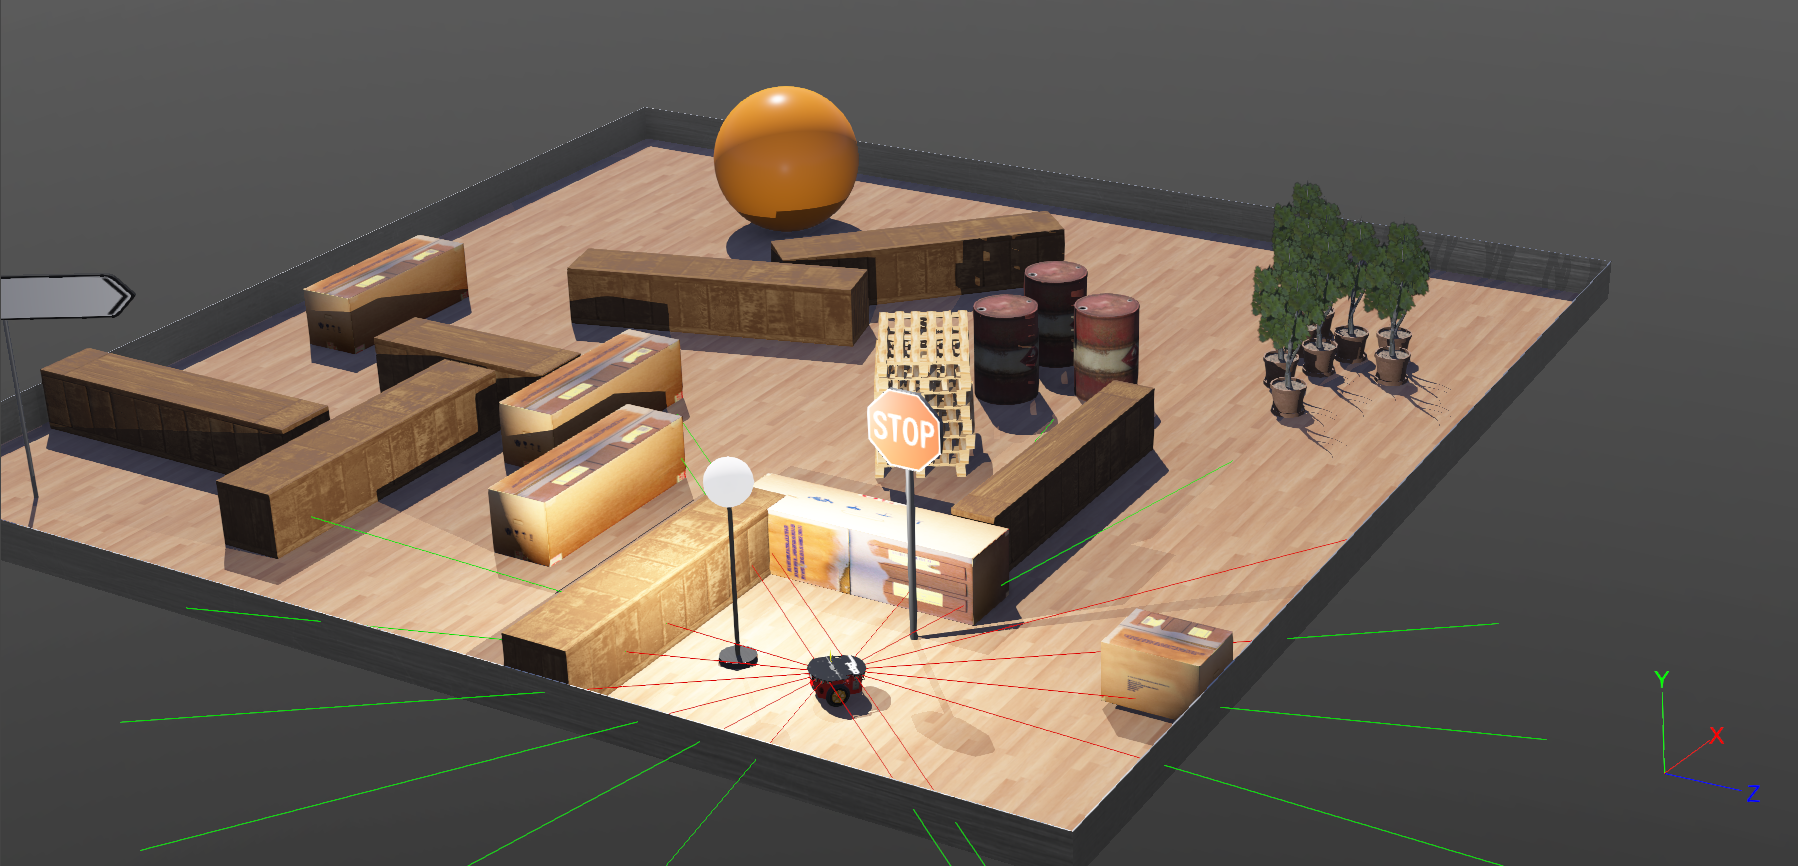
\includegraphics[width=1\textwidth]{Figures/webots3.png}
    \caption*{Fonte: Autoria propria.}
    \label{fig:Webots}
\end{figure}


\section{Desafio Husky}
Husky é um veiculo UGV no qual atraves do ROS pode ser 
simulado em conjunto com o gazebosim e o rviz, sendo ambos
simualdores no qual o primeiro é voltado para o ambiente 
ao redor do husky e o segundo é como esse ugv percebe o mundo.
O desafio consiste em utilizar os simuladores para testar
diferentes formas de navegação com o husky.

O primeiro desafio é simular o husky com o package move base. 
Consiste em dar uma localização no mundo e ele ira tentar atingir 
esse objetivo. Caso o ugv identifique algum obstaculo ele ira desviar,
ou caso fique preso ira entrar em um processo chamado conservative reset
se parar de ficar preso voltara a navegação, caso não entrara em 
clearing rotation, se mesmo assim continuar preso iniciara um agressive reset
e continuando preso vai por fim fazer uma clearing rotation e se mesmo 
assim continuar preso vai abortar a ação. Como mostra na imagem \ref{fig:Move Base}.

%imagem https://wiki.ros.org/move_base

\begin{figure} [h!]
    \centering
    \caption{Move Base}
    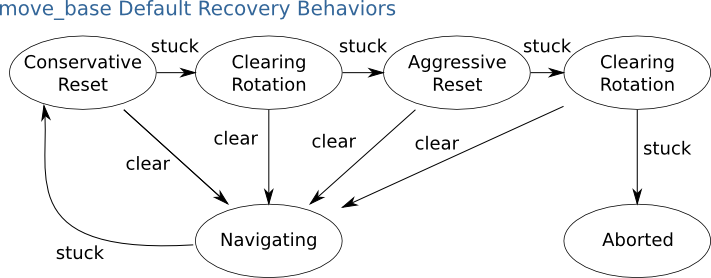
\includegraphics[width=0.8\textwidth]{Figures/recovery_behaviors.png}
    \caption*{Fonte: ROS Wiki.}
    \label{fig:Move Base}
\end{figure}

O segundo desafio é o amcl demo, o qual é a junção do move base com o
amcl. Assim o amcl é um sistema probabilistico de localização do robô
o qual atraves de sensores de laser fazem o tracking da posisção do 
robo dentro de um mapa.

%imagem do simulador 

Gmapping demo é o terceiro desafio, ele é a junção do move base com o
gmapping. Esse package prove um SLAM (Simultaneos localization and mapping), 
baseado em sensores a laser. Com o gmapping é criado um mapa 2D do ambiente.
Como pode ser mostrado na imagem abaixo.

%imagem do mapa

Por ultimo foi realizado o frontier exploration demo, é composto 
pelo move base, gmapping, e o frontier exploration. Dessa forma,
o frontier em conjunto com esses packages para realizar a 
exploração de ambientes

%----------------------------------------------------------

%--------- NEW SECTION ----------------------


%---------------picture------------------------------------
% \begin{figure}
%     \centering
%     \subfigure[Figure A]{\label{fig:a}\includegraphics[width=60mm]{./lq}}
%     \subfigure[Figure B]{\label{fig:b}\includegraphics[width=60mm]{./lq}}
%     \subfigure[Figure C]{\label{fig:c}\includegraphics[width=\textwidth]{./lq}}
%     \caption{Three simple graphs}
%     \label{fig:three graphs}
% \end{figure}
%----------------------------------------------------------

% \begin{figure}
%     \centering
%     \begin{subfigure}[b]{0.3\textwidth}
%         \centering
%         \includegraphics[width=\textwidth]{./lq}
%         \caption{$y=x$}
%         \label{fig:y equals x}
%     \end{subfigure}
%     \hfill
%     \begin{subfigure}[b]{0.3\textwidth}
%         \centering
%         \includegraphics[width=\textwidth]{./lq}
%         \caption{$y=3sinx$}
%         \label{fig:three sin x}
%     \end{subfigure}
%     \hfill
%     \begin{subfigure}[b]{0.3\textwidth}
%         \centering
%         \includegraphics[width=\textwidth]{./lq}
%         \caption{$y=5/x$}
%         \label{fig:five over x}
%     \end{subfigure}
%        \caption{Three simple graphs}
%        \label{fig:three graphs}
% \end{figure}


% %--------- NEW SECTION ----------------------
% \section{Assunto 2}
% \label{sec:ass2}
% flkjasdlkfjasdlkfjs

% \begin{table}[h]
%     \begin{subtable}[h]{0.45\textwidth}
%         \centering
%         \begin{tabular}{l | l | l}
%         Day & Max Temp & Min Temp \\
%         \hline \hline
%         Mon & 20 & 13\\
%         Tue & 22 & 14\\
%         Wed & 23 & 12\\
%         Thurs & 25 & 13\\
%         Fri & 18 & 7\\
%         Sat & 15 & 13\\
%         Sun & 20 & 13
%        \end{tabular}
%        \caption{First Week}
%        \label{tab:week1}
%     \end{subtable}
%     \hfill
%     \begin{subtable}[h]{0.45\textwidth}
%         \centering
%         \begin{tabular}{l | l | l}
%         Day & Max Temp & Min Temp \\
%         \hline \hline
%         Mon & 17 & 11\\
%         Tue & 16 & 10\\
%         Wed & 14 & 8\\
%         Thurs & 12 & 5\\
%         Fri & 15 & 7\\
%         Sat & 16 & 12\\
%         Sun & 15 & 9
%         \end{tabular}
%         \caption{Second Week}
%         \label{tab:week2}
%      \end{subtable}
%      \caption{Max and min temps recorded in the first two weeks of July}
%      \label{tab:temps}
% \end{table}